\chapter{径流模型CaMa-Flood}
%\addcontentsline{toc}{chapter}{陆地表面的水分循环}

汇流计算是通过耦合 Dai Yamazaki 等人于2011年提出的大尺度分布式汇流模型 CaMa-Flood (Catchment-based Macro-scale Floodplain) 实现的\citep{yamazaki2011physically}。
CaMa-Flood将全球河流网络分割为称为流域单元 (unit catchment) 的水文单元,在各单元集水区内利用河道 (river channel) 和漫滩 (floodplain) 的次网格 (subgrid) 
地形参数以及陆面模式生成的产流量 (total runoff),对总蓄水量 (total storage) 以及总流量 (total discharge) 进行预测,
并进一步实现对河道及漫滩流量 (river discharge and flood discharge),漫滩面积 (flood area) 以及平均漫滩水深 (flood depth) 
等日常所需的诊断量的高速计算。总蓄水量和总流量的时间演变通过求解局部惯性方程 \citep{bates2010} 得出。
CaMa-Flood同时考虑了上游单元的入流、下游单元的流出和每个流域单元的径流强迫输入,是目前高速求解河道水动力方程-圣维南方程最为高速有效的方法之一。
关于CaMa-Flood模型的详细描述可以从相关文献获取\citep{yamazaki2011physically,yamazaki2013improving,yamazaki2014regional,yamazaki2014development}。


CaMa-Flood 模型的主要优势之一在于除了能够精确描述河道径流以外,还能够模拟包括漫滩水位和漫滩面积变化等洪泛过程。
因此,对模拟结果的验证不仅仅局限于传统测量河流流量,还可以直接将模拟结果与卫星高度计对水面高程的观测以及微波成像仪对洪泛面积的估算进行比较;
能够有效加强全球河流模型各个输出的校准/验证\citep{yamazaki2012adjustment,yamazaki2012analysis}。
CaMa-Flood 模型的另一个优势在于它具有极高的模拟计算效率。通过引入次网格地形参数,复杂的漫滩淹没物理过程被合理地简化。
与此同时,通过实现局部惯性方程和自适应时间步长等物理方案\citep{bates2010},
河流流量和蓄水量的预测计算成本得到压缩,有利于进行集成/长期实验等计算要求高的实验或者与陆面模式之间的动态耦合。
以下对 CaMa-Flood 内部各个模块进行详细的介绍。目前耦合版本陆面过程模式分系统已经包含 CaMa-Flood v4.07版本。



\section{诊断洪泛状态}\label{诊断洪泛状态}
在 CaMa-Flood 中指定网格的漫滩 (洪泛) 状态是通过计算该网格的蓄水总量得出的。如图~\ref{fig:CaMa-Flood流域单位示意图}
所示,河流河道蓄水量$S_r$,漫滩蓄水量$S_f$,河道水深度$D_r$, 漫滩淹没深度$D_f$,漫滩面积$A_f$等均通过求解基于总蓄水量的水量方程得出。
首先,模式中引发当前流域单元洪水蓄水量$S_{ini}$由如下公式进行确定:
\begin{equation}
S_{ ini }=B WL
\end{equation}
其中$B$是河道深度,$W$是河道宽度,及$L$是河道长度。如果总蓄水量$S$小于等于引发洪水蓄水量$S_{ini}$,
CaMa-Flood 假设不存在漫滩 (洪泛) 事件,上述参数则通过如下方程计算得出:
\begin{equation}
    \begin{array}{l}S_r=S \\ D_r=\frac{S_r}{WL} \\ S_f=0 \\ D_f=0 \\ A_f=0 \\ S_f=0\end{array}
\end{equation}
当总蓄水量$S$大于引发洪水蓄水量$S_{ini}$时,触发漫滩 (洪泛) 事件,则上述参数通过联立如下方程计算得出:
\begin{equation}
\begin{array}{l}S_r=S-S_f \\ D_r=\frac{S_r}{W L} \\ S_f=\int_{0}^{A_f}(D_f-D(A)) d_A \\ D_f=D_r-B \\ A_f=D^{-1}(D_f)\end{array}
\end{equation}
上式中的$D_f = D_r - B$表示河道与漫滩的水面高度相同。该方程是基于河道与漫滩之间的水量瞬间完成交换的假设。
函数$D^{-1}(D_f)$是漫滩高程剖面$D(A_f)$的反函数,它将泛滥地区$A_f$描述为漫滩水深$D_f$的函数 (见图~\ref{fig:CaMa-Flood流域单位示意图})。


{
\begin{figure}[]
\centering
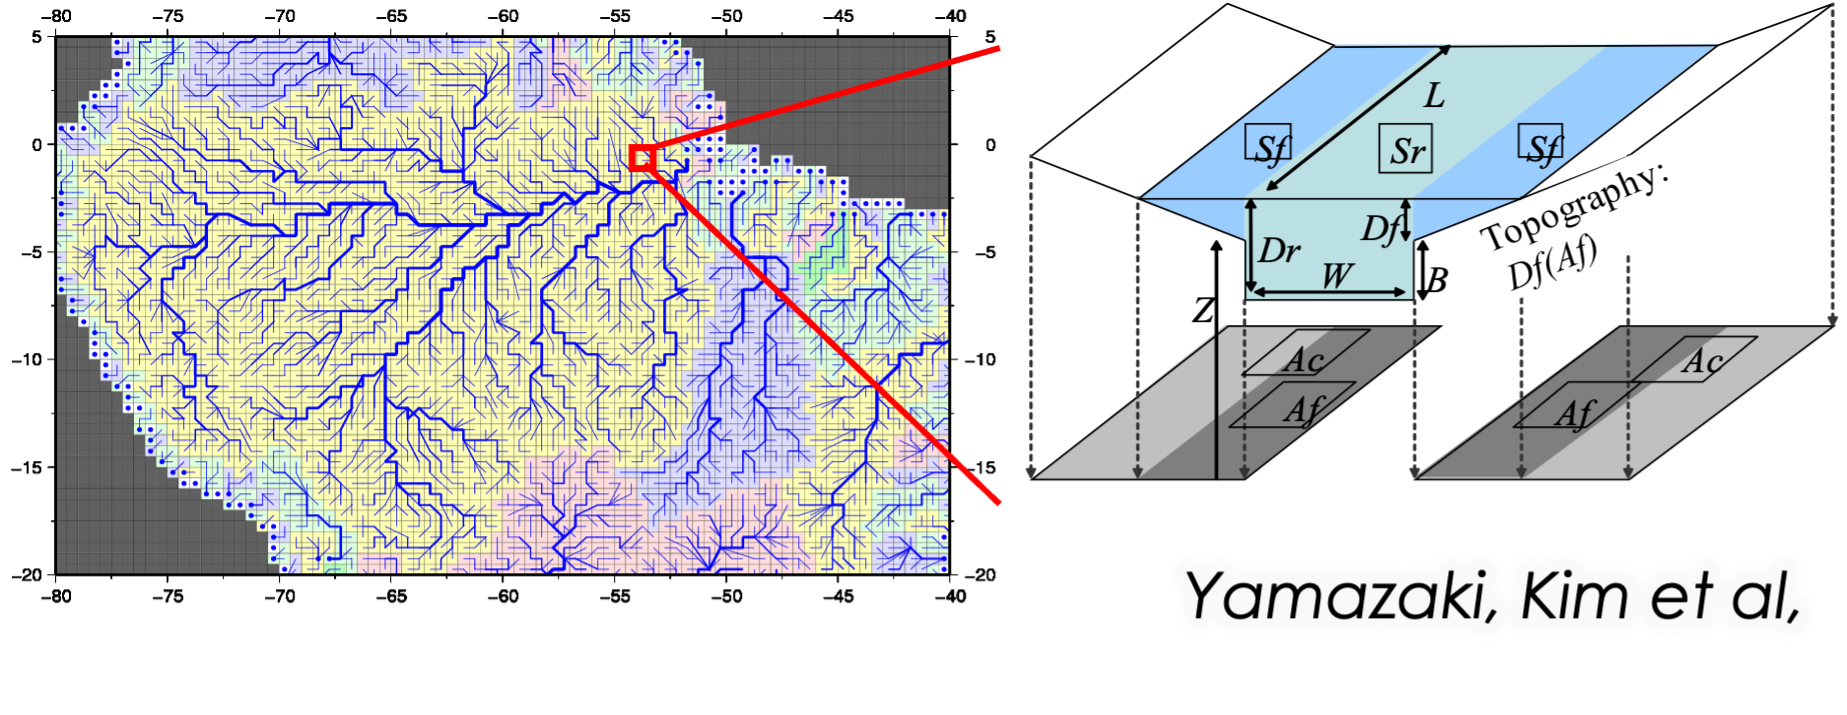
\includegraphics{Figures/陆地表面的水分循环/CaMa-Flood流域单位示意图.png}
\caption{CaMa-Flood流域单位示意图,摘自\citet{yamazaki2011physically}。 }
\label{fig:CaMa-Flood流域单位示意图}
\end{figure}
}

\section{河道径流流量计算}
CaMa-Flood 分别计算了各流域单元向其下游单元的河流径流量和漫滩流量。
二者的计算均通过忽略如下 St. Venant 动量方程式第二项,得到径流计算所使用的局部惯性方程 \cite{bates2010}:
\begin{equation}
\frac{\partial Q}{\partial t}+\frac{\partial}{\partial x}\left[\frac{Q^{2}}{A}\right]+\frac{g A \partial(h+z)}{\partial x}+\frac{g n^{2} Q^{2}}{R^{4 / 3} A}=0
\end{equation}
式中$Q$为河流流量 (\unit{m^3.s^{-1}}),$A$为水流横截面面积 (\unit{m^2}),$h$为水流深度 (m),$z$为河床高程 (m),
$R$为水力半径 (m),$g$为重力加速度 (\unit{m.s^{-2}}),$n$为曼宁摩擦系数(\unit{m^{-1/3}.s^{-1}})。
$x$和$t$分别为流动距离和时间。第一项、第二项、第三项和第四项分别表示局部加速度、平流、水面坡度和摩擦坡度。CaMa-Flood模型采用局部惯性方程的显式形式: 

\begin{equation}
Q^{t+\Delta t}=\frac{Q^{t}+\Delta t g A i S}{1+\frac{\Delta t g n^{2}\left|Q^{t \mid}\right|}{R^{4 / 3} A}}
\end{equation}
其中$S$是水面坡度,$Q^t$为当前时刻的流量, $Q^{t+\Delta t}$是单位时间间隔 $\Delta t$ 之后的流量。水力半径 $R$ 近似为水流深度。曼宁系数默认设置为$n=0.03$。
在局部惯性方程计算中可能出现的负向河流量,代表了下游流域单元向当前流域单元的反向水流(回水)。同时为防止当前网格的总的流出量超过蓄水量,
CaMa-Flood 引入限流器的概念:当总出水量大于网格的总库存量时,CaMa-Flood 使用修正系数对径流流量进行修正。


\section{洪水漫滩流量计算}
漫滩流量计算与河道径流流量计算方法相同。
其区别在于漫滩流量包括所使用的水流面积$A$的计算方法是漫滩蓄水量除以河道长度;
水流深度$h$为漫滩深度;漫滩流量的曼宁系数被设置为$n=0.10$。

\section{蓄水量变化计算}
{
\begin{figure}[]
\centering
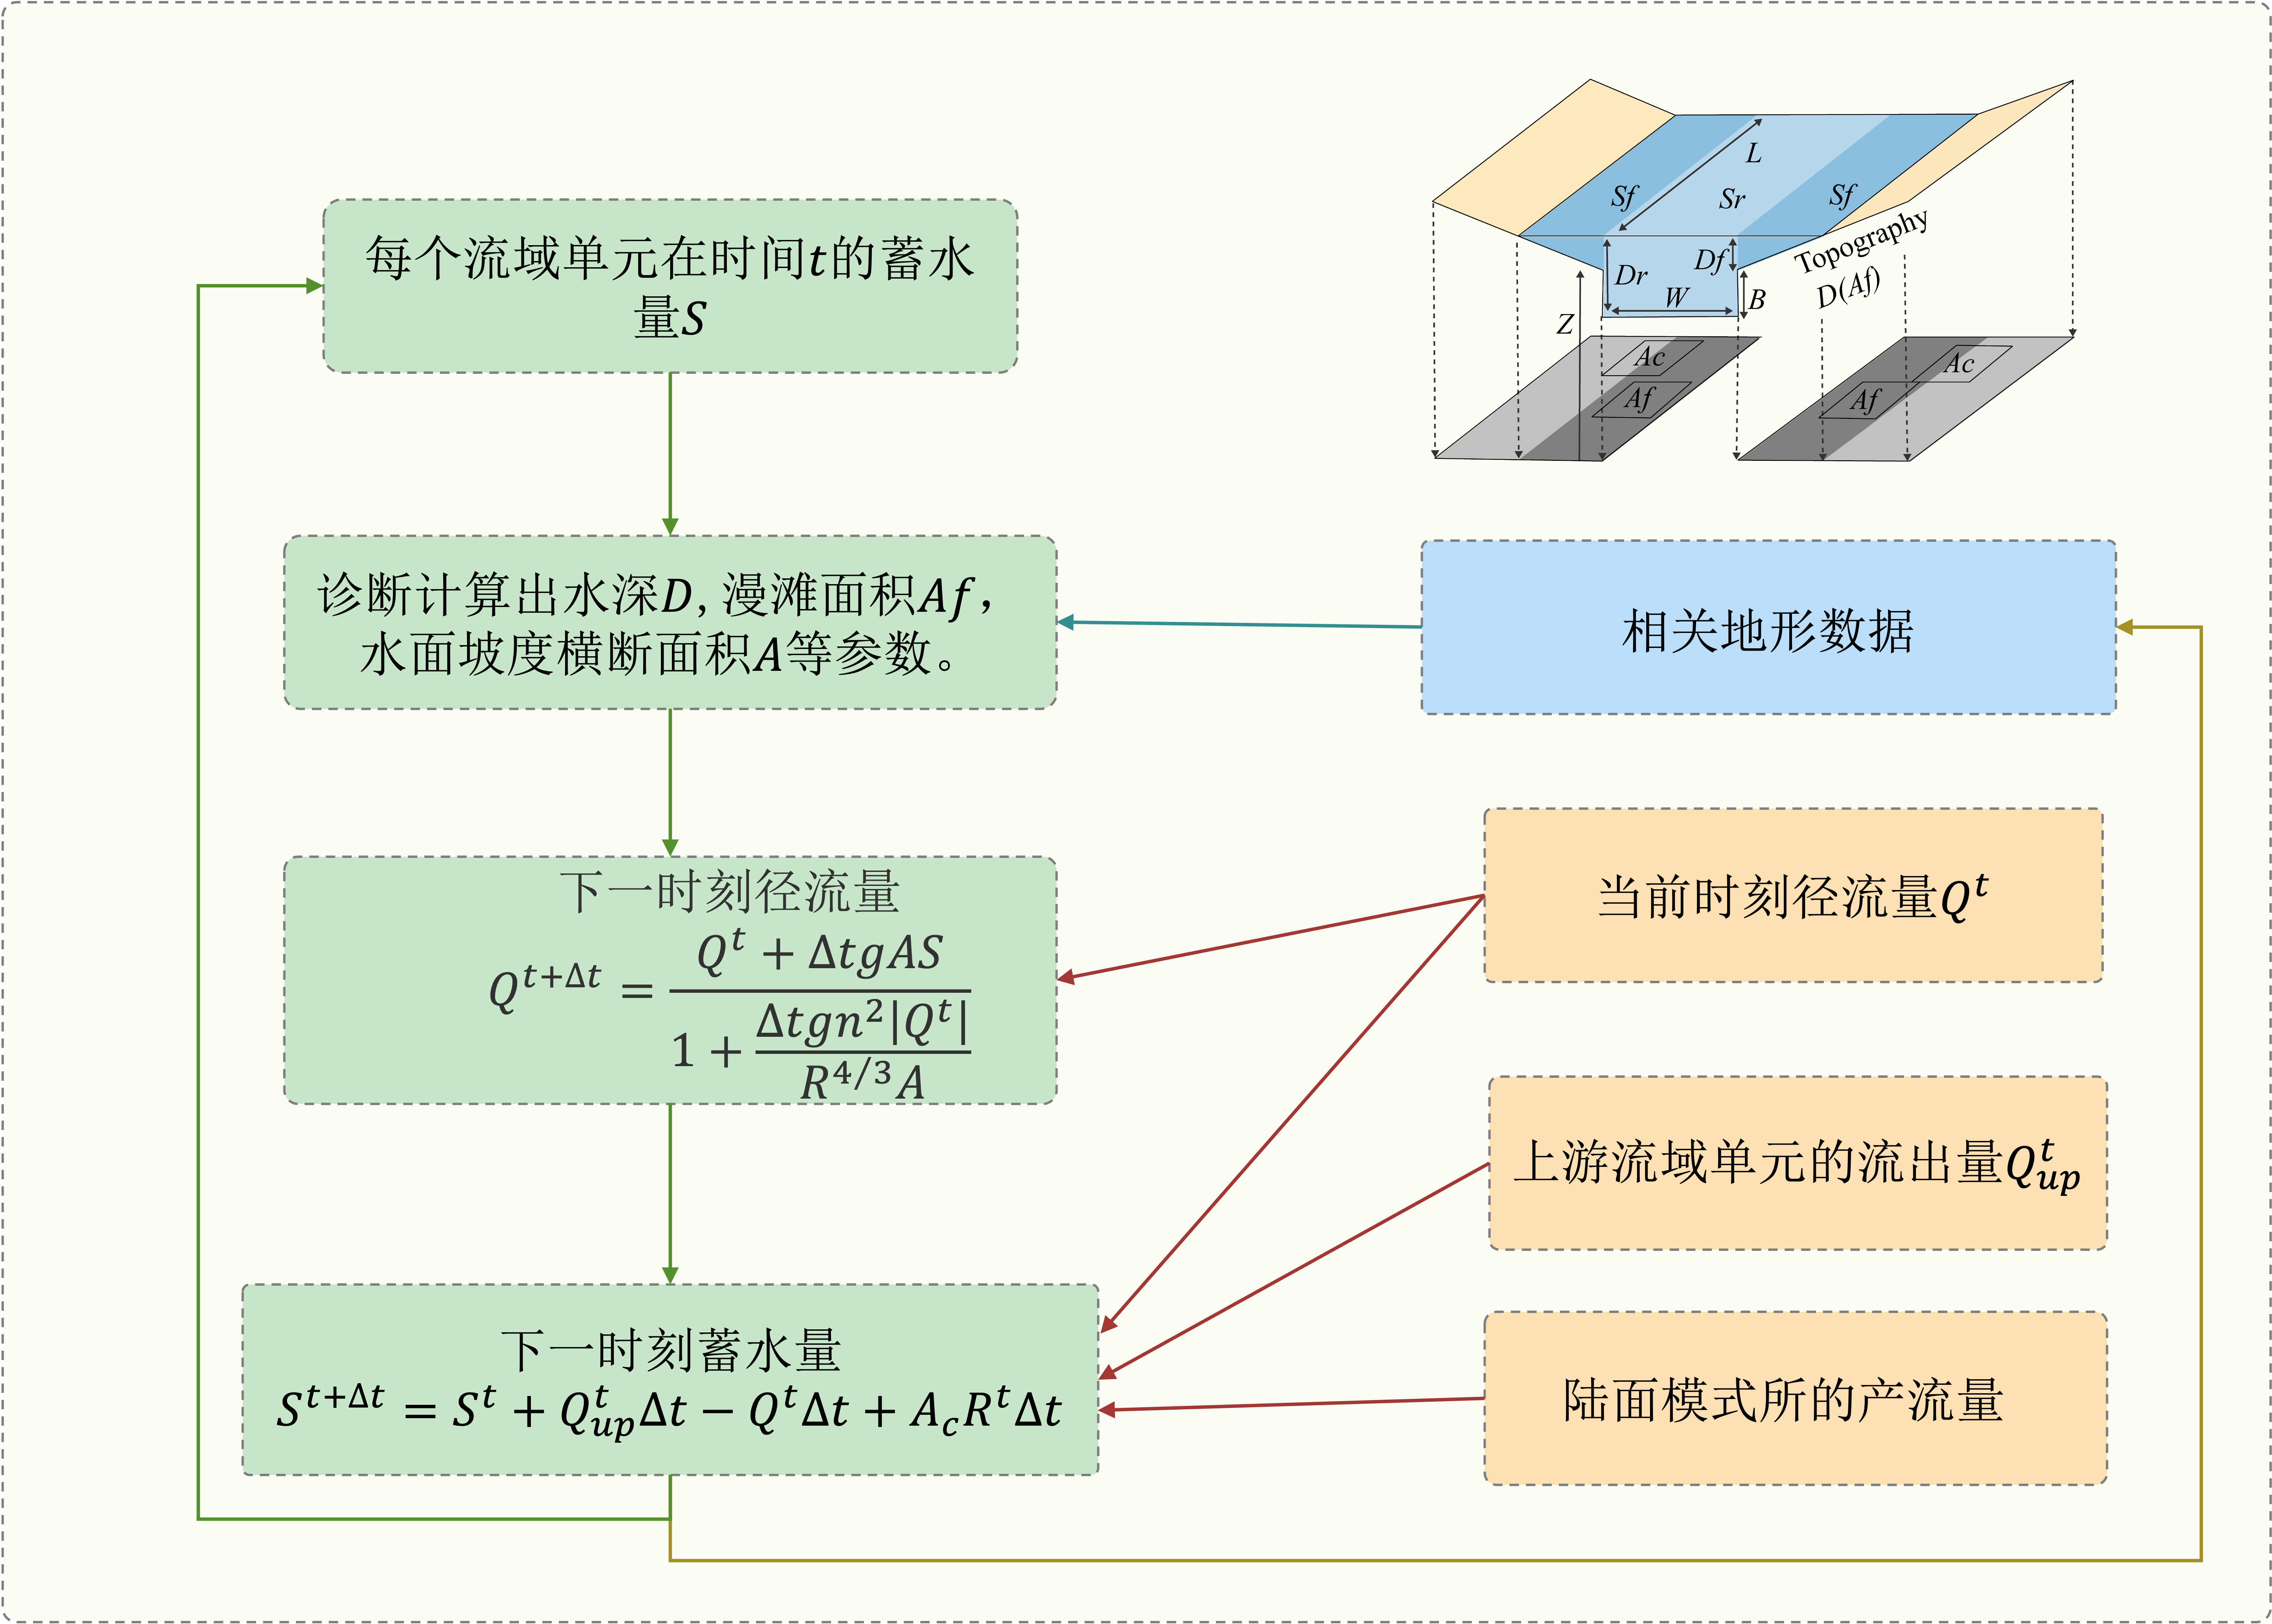
\includegraphics{Figures/陆地表面的水分循环/蓄水量变化计算流程图.png}
\caption{蓄水量变化计算流程图。 }
\label{fig:蓄水量变化计算流程图}
\end{figure}
}
蓄水量随时间的变化的计算流程如图~\ref{fig:蓄水量变化计算流程图} 所示,指定流域单元的蓄水量变化的计算基于质量平衡方程:
\begin{equation}
S_{i}^{t+\Delta t}=S_{i}^{t}+\sum_{k}^{Upstream} Q_{k}^{t} \Delta t-Q_{i}^{t} \Delta t+A c_{i} R_{i}^{t} \Delta t
\end{equation}
式中$S_{i}^{t}$和$S_{i}^{t+\Delta t}$分别代表单元$i$在时间$t$到时间$t+\Delta t$蓄水量的变化,$Q_i^t$代表在时间$t$该单元河流径流出流量 (河道内+漫滩),
$Q_k^t$代表在时间 $t$ 该单元从上游网格接收的河流径流流入流量 (河道内+漫滩),$Ac_i$ 是单元$i$的面积,$R_i^t$ 代表流域单元 $i$ 的产流量。

\section{自适应时间步长的估算}
为避免固定时间步长计算所产生的数值振荡,提高数值方案稳定性,
CaMa-Flood 采用了\citet{bates2010}提出的基于局部惯性方程并满足 Courant-Friedrichs-Lewy (CFL) 
条件的自适应时间步长 ($DT_{adp}$) 的估算方法:
\begin{equation}
{DT}_{\max }=\boldsymbol{\alpha} \frac{\Delta x}{\sqrt{g h_{t}}}
\end{equation}
上式中$DT_{max}$是最大可接受的时间步长,$∆x$是该流域单元连接下游流域单元的河道长度 (river length) (m),
$\alpha$是稳定性系数设为0.9,$h_t$是该流域单元在时刻$t$的水流深度 (water depth) (m),$g$是重力加速度设为9.81 (\unit{m.s^{-2}})。
图~\ref{fig:自适应时间步长的估算} 展示了基于上述公式计算的某一时刻的$DT_{max}$ (minute)。
在计算过程中,如果用户指定的默认时间步长$DT$大于$DT_{max}$,则$DT$将被划分为满足$CFL$条件的更小的时间等分的时间步长$DT_{adp}$;
如果用户指定的默认时间步长$DT$小于$DT_{max}$,则实际计算步长按照用户指定的默认时间步长。
{
\begin{figure}[]
\centering
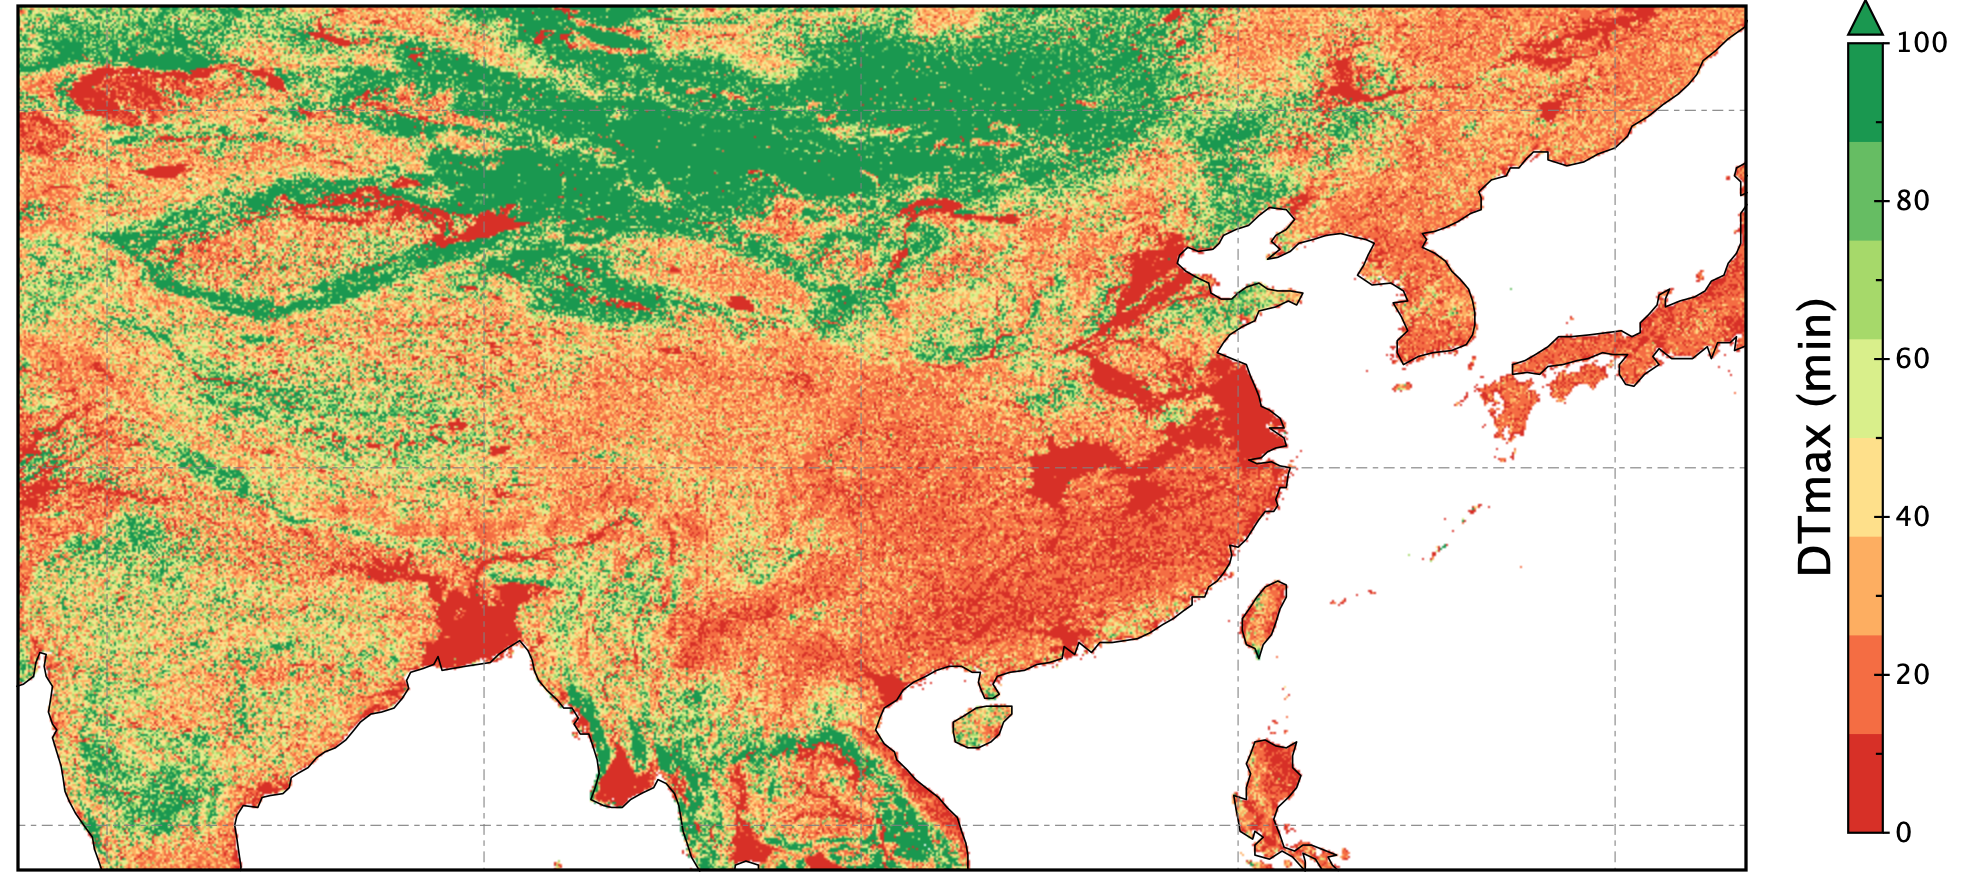
\includegraphics{Figures/陆地表面的水分循环/自适应时间步长的估算.png}
\caption{自适应时间步长的估算,摘自\citet{yamazaki2013improving}。}
\label{fig:自适应时间步长的估算}
\end{figure}
}
